\documentclass[12pt]{article}
\usepackage{amsmath,amssymb,amsthm}
\usepackage[margin=1in]{geometry}
\usepackage{tikz,fancyhdr,enumerate,graphicx,subcaption}
\usepackage[inline]{enumitem}
\usepackage[labelfont=bf]{caption}

\pagestyle{fancy}
\fancyhf{}
\chead{PROBLEM SET 2}
\rhead{Elliot Ahn}
\rfoot{\thepage}
\lhead{CS155}

\setlength{\headheight}{15pt}
\renewcommand{\footrulewidth}{0.5pt}

\newcommand{\E}{\mathbb E}
\newcommand{\Eout}{E_{\text{out}}}
\newcommand{\x}{\mathbf x}
\newcommand{\w}{\mathbf w}
\newcommand{\y}{\mathbf y}
\newcommand{\X}{\mathbf X}

\begin{document}

\begin{enumerate}[leftmargin=*]
\item
\begin{enumerate}[label = \Alph*.]
\item Squared loss tends to be very bad for classification because we only have two target values $y \in \{-1, +1\}$ whereas the predicted value $w^T x_i$ can be any real value. Therefore, it is very unlikely that the regression will give $y = \pm 1$ and the squared error will not capture what we're looking for.
\item The main qualitative difference between the two separating boundaries is the slope of the line. The linear fit seems to have the line more perpendicular to the data while the logistic regression boundary is more steep.

An explanation is that for logistic regression, cross-entropy error minimization is equivalent to likelihood-maximization, where the target values are interpreted as probabilities. Clearly, the MLE in the data above is a step function dividing the classes. However, in a step function, the weight $||w|| \to \infty$, and with regularzation, we must bound the magnitude of the weights. For the regularization parameter that scikit-learn uses, the boundary turns out to be this.

As we said before in part A, squared-error minimization is a poor choice for classification, and so it happens that the boundary does not separate our separable data. However, due to the symmetry of problem, the ridge regression keeps the boundary line approximately perpendicular to the data points.
\begin{figure}[h]
\centering
\begin{subfigure}[t]{0.45\textwidth}
\centering
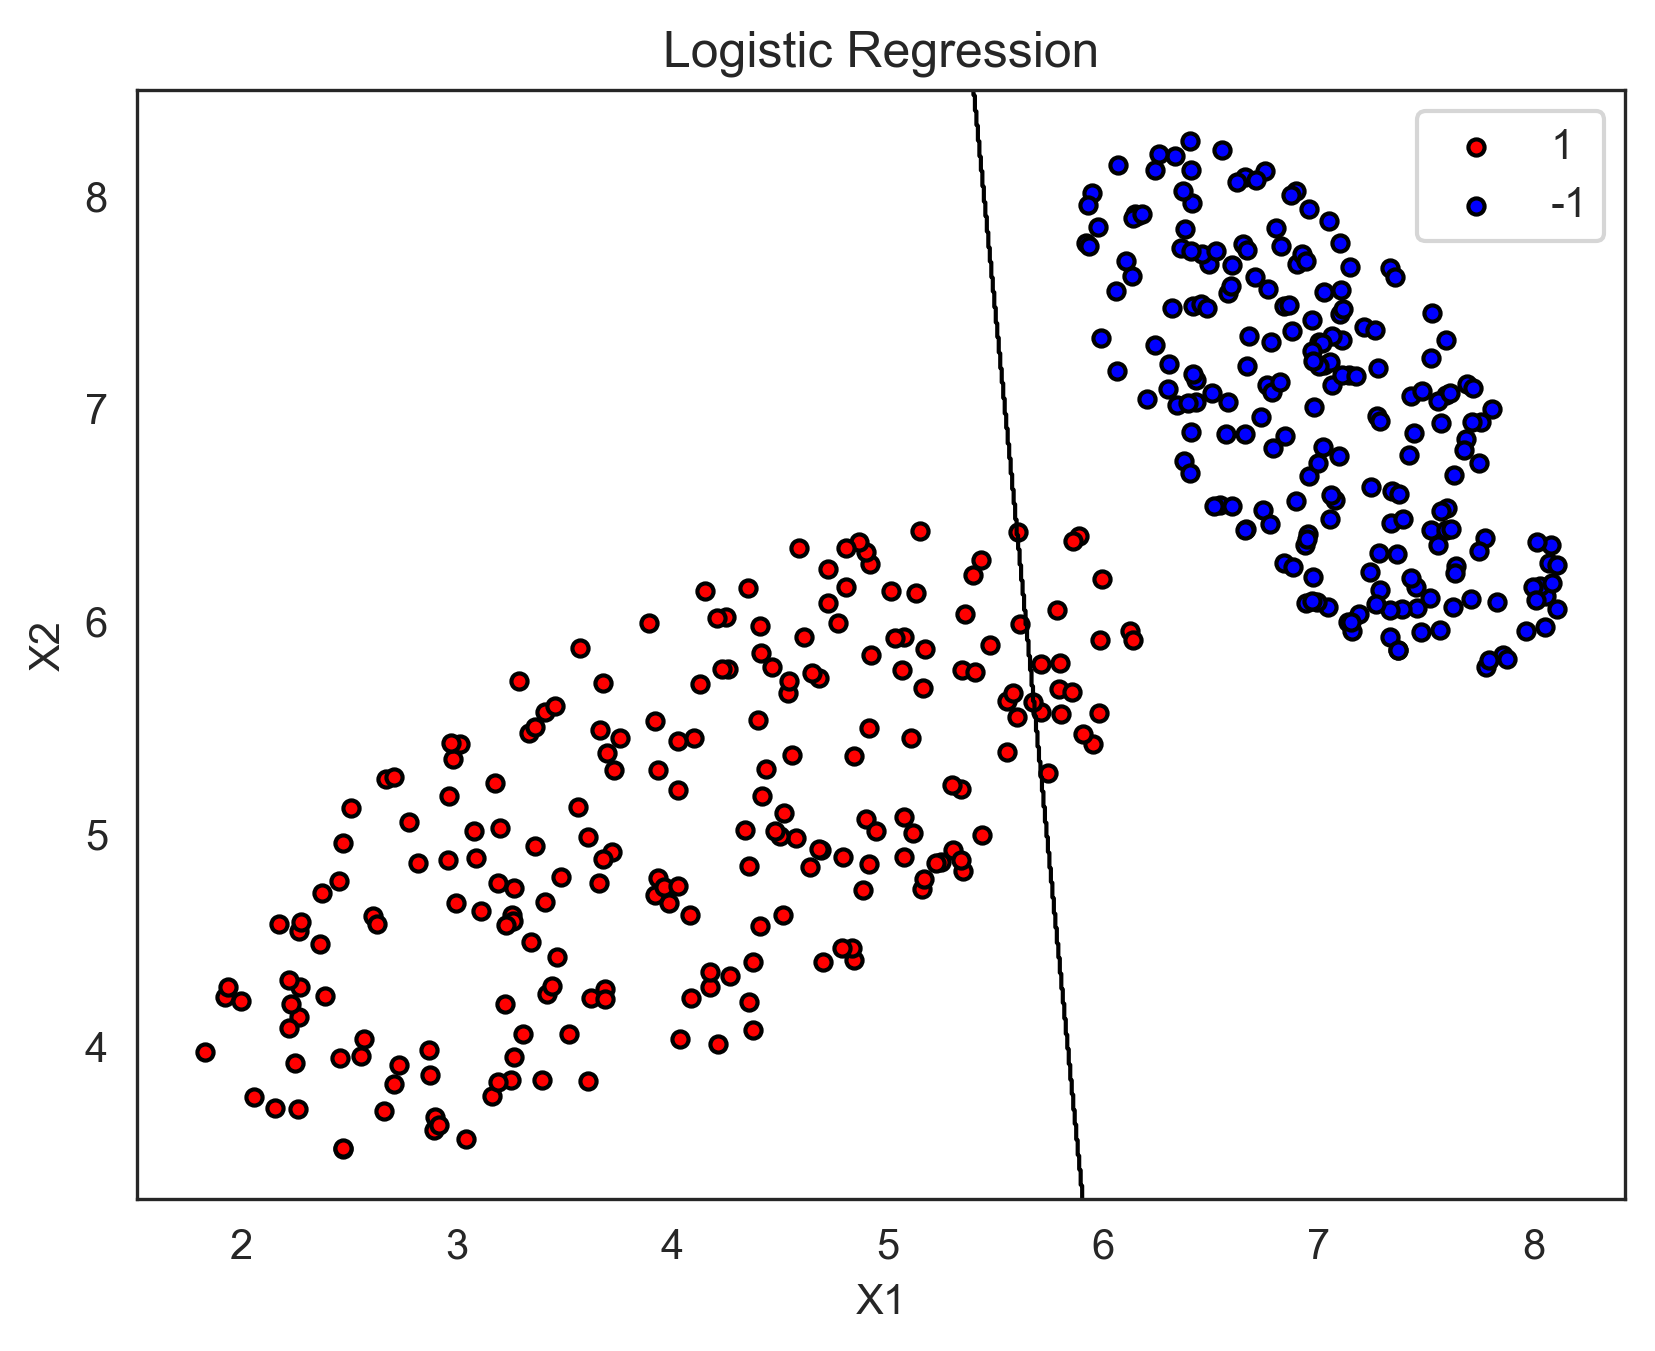
\includegraphics[scale=0.5]{logregress.png}
\caption{Cross-Entropy Error}
\end{subfigure}
~
\begin{subfigure}[t]{0.45\textwidth}
\centering
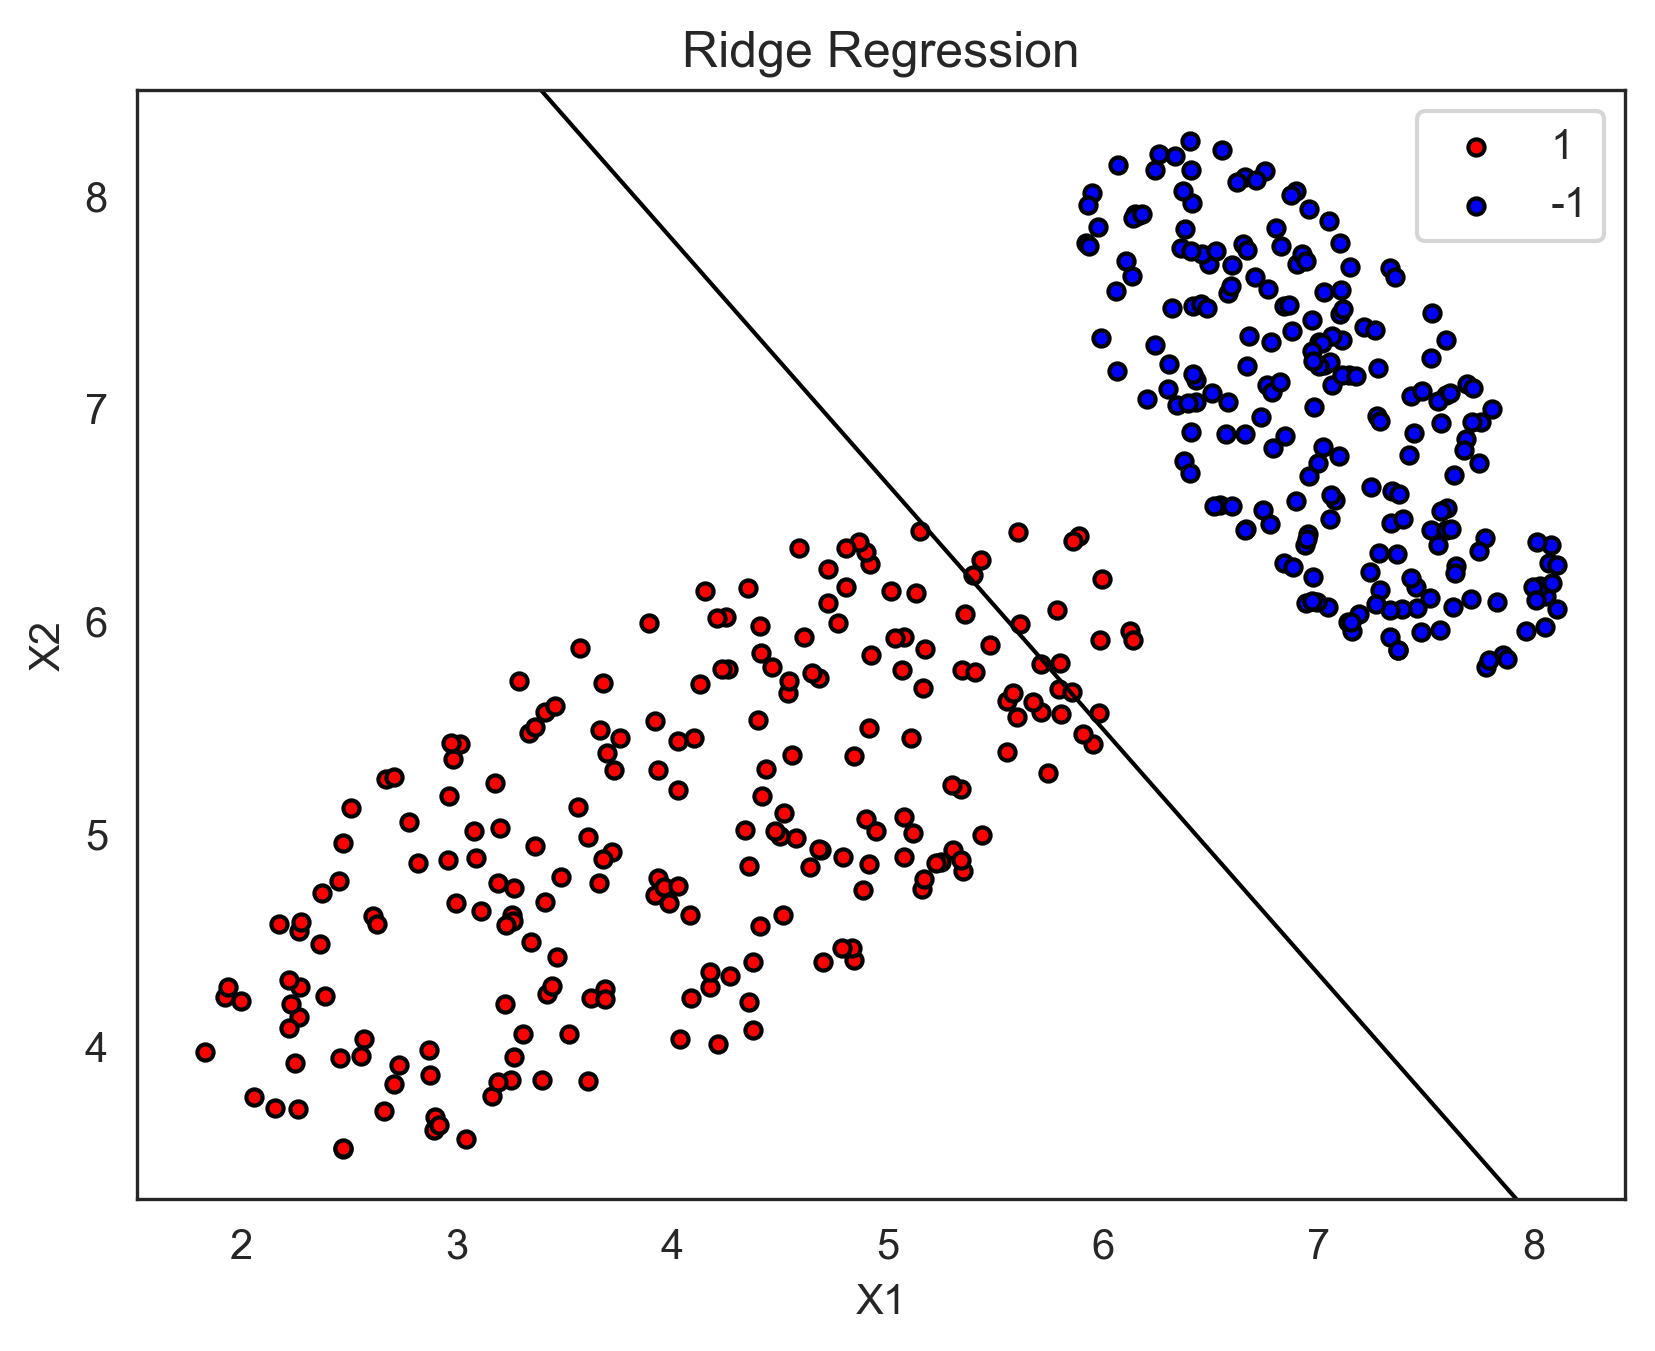
\includegraphics[scale=0.5]{ridregress.png}
\caption{Squared Error}
\end{subfigure}
\end{figure}
\item We have (with regularization)
\[ \nabla_w L_{\text{log}} = \frac{1}{2} \lambda \w - \frac{y \x}{1 + e^{y \w^T \x}}, \qquad \nabla_w L_{\text{hinge}} = \frac{1}{2} \lambda \w + \begin{cases} 0 & y \w^T \x > 1 \\ -y \x & y \w^T \x \leq 1 \end{cases} \]

For the points in $S$, we have the table shown below.
\begin{center}
\begin{tabular}{|c c c|}
\hline
$S$ & $\nabla_w L_{\text{log}}$ & $\nabla_w L_{\text{hinge}}$ \\ \hline
(1/2, 3) & (-0.38, -0.19, -1.13) & (-1, -0.5, -3) \\
(2, -2) & (-0.12, -0.24, 0.24) & (0, 0, 0) \\
(-3, 1) & (0.047, -0.14, 0.047) & (0, 0, 0) \\ \hline
\end{tabular}
\end{center}
\item For the log loss, without regularization ($\lambda = 0$), we can never get a case where $\nabla_w L_{\text{log}} = 0$ unless the weights go to infinity, in which case the weights don't converge. For the hinge loss, we can get a case where $\nabla_w L_{\text{hinge}} = 0$ if all the points satisfy $y \w^T \x > 1$. If we get a point that doesn't satisfy the condition, then the next iteration yields
\[ \w \to \w + \eta y \x \implies y \w^T \x' \to y(\w + \eta y \x)^T \x' = y \w^T \x' + \eta \x^T \x' \]
For the corrected point where $\x' = \x$, we see that $\eta \x^T \x > 0$ so that our margin $y \w^T x$ increases and at some point surpasses $1$ so that our hinge gradient is zero.

Thus, for a linearly separable dataset, the cross-entropy error will never be zero because the weights have to diverge. For hinge-loss, the training error could become zero.
\item SVM is a ``maximum margin'' classifier because the motivation for SVM is to maximize the margin between the classes. By normalizing $|\w^T \x| = y \w^T \x =1$ at the margin, this problem becomes equivalent to maximizing $1 / |w|$. This is equivalent to minimizing
\[ \frac{1}{2} \w^T \w \qquad \text{subject to} \qquad y \w^T \x \geq 1. \]
Using Lagrange multipliers, we want to minimize the following Lagrangian,
\[ \mathcal L = \frac{1}{2} \w^T \w - \sum_n \alpha_n (y_n \w^T \x_n - 1). \]
If we impose soft constraints where we can violate the margin at a certain cost, we have
\[ y_n \w^T \x_n \geq 1 - \xi_n, \qquad \xi_n \geq 0 \]
where $\xi_i$ is the margin violation. We impose a cost, $C$, where we now impose the minimization
\[ \mathcal L = \frac{1}{2} \w^T \w + C \sum_n \xi_n - \sum_n \alpha_n (y_n \w^T \x_n - 1 + \xi_n) - \sum_n \beta_n \xi_n \]
We see that we can interpret the above Lagrangian as trying to minimize the hinge loss $\xi_n$ with respect to some constraints as well as adding a regularization on $\w$ with $\lambda = 1$.
\end{enumerate}
\item
\begin{enumerate}[label = \Alph*.]
\item No, adding a penalty term cannot decrease in-sample error because in-sample error is always directly minimized. Adding a penalty term, however, does not always decrease out-of-sample error. A large penalty can cause underfitting which can hurt out-of-sample error.
\item We don't use $\ell_0$ regularization because
\[ ||w||_0 = \sum_d 1_{[w_d \neq 0]} \]
is not continuous and thus is difficult to computationally optimize. Also, $\ell_1$ is sparse enough and continuous.
\item We can see how different $\lambda$'s affect our training in the following three figures.
\begin{figure}[h!]
\centering
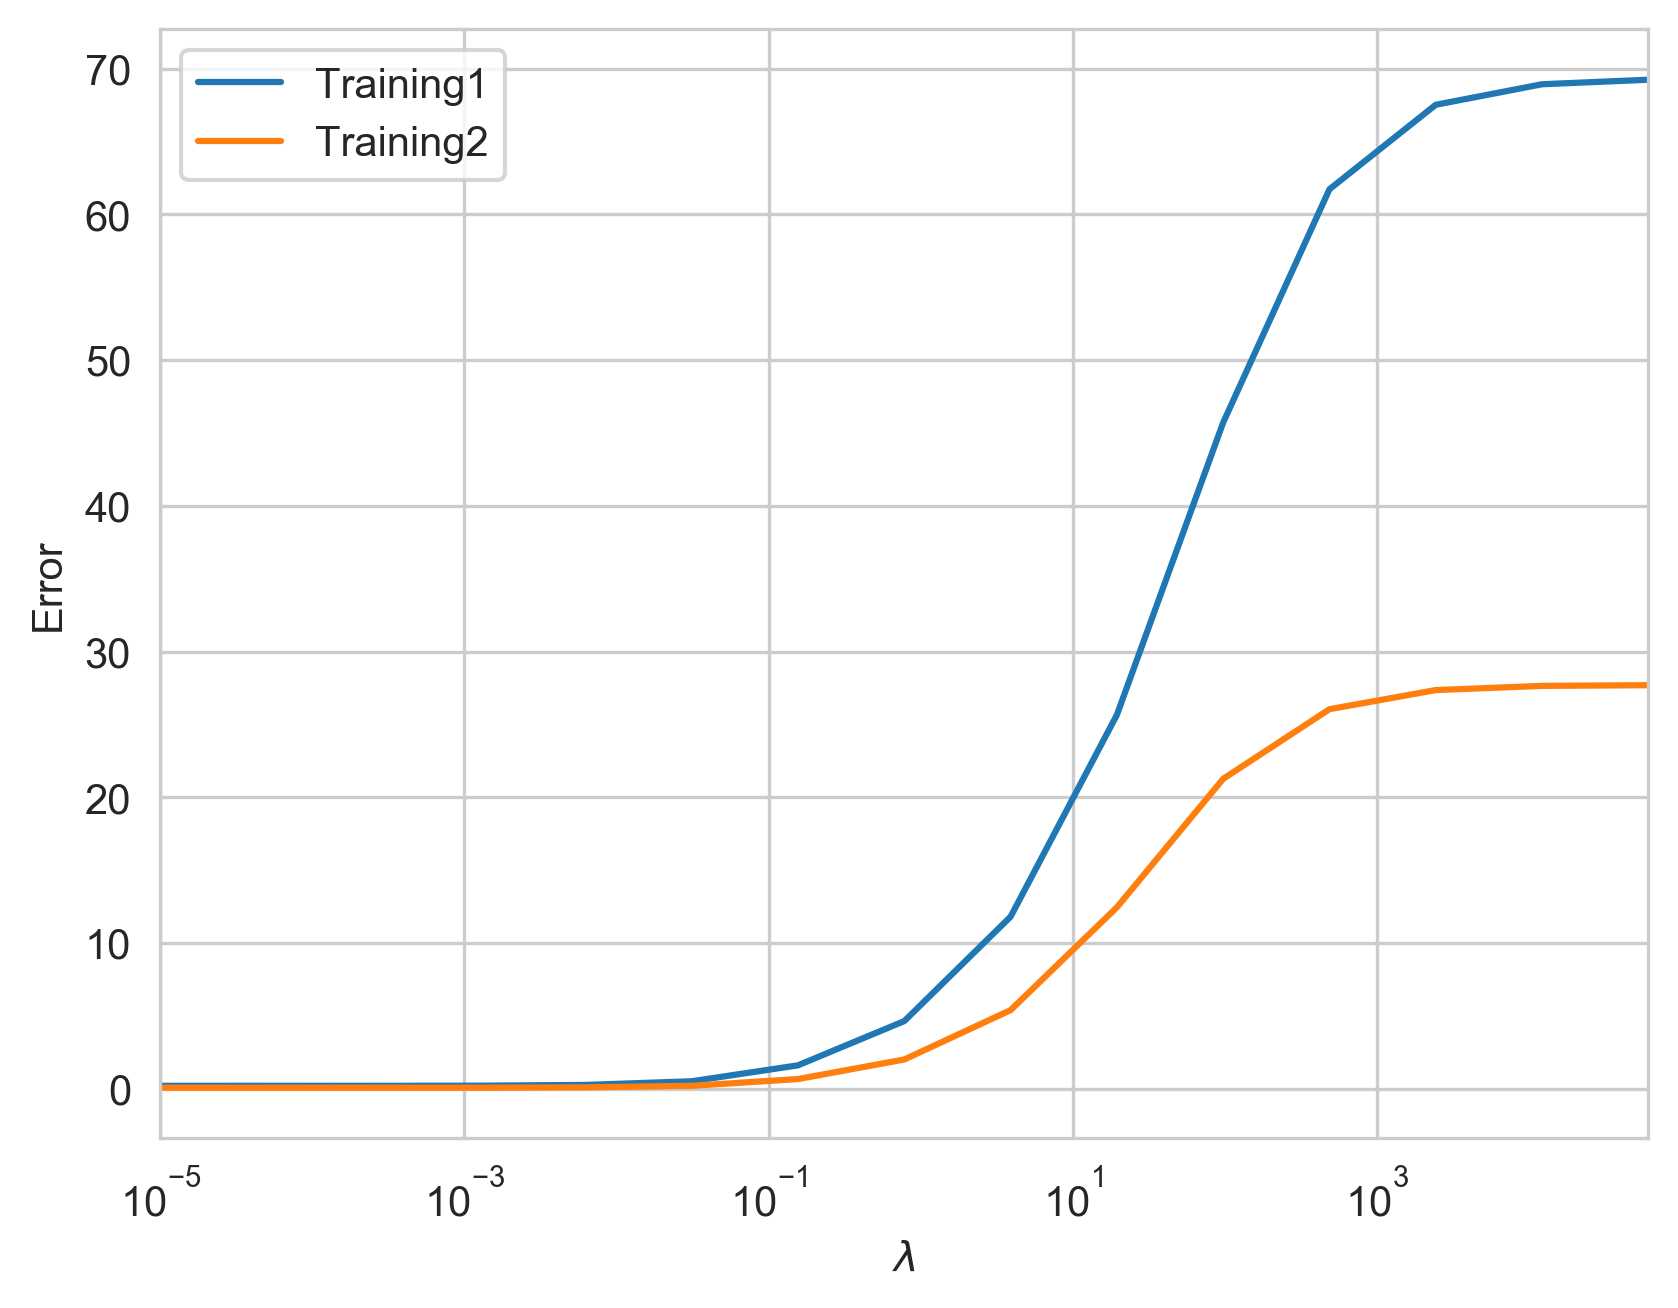
\includegraphics[scale=0.56]{regEin.png}
\caption{In-sample error for different $\lambda$'s.}
\end{figure}

\begin{figure}[h!]
\centering
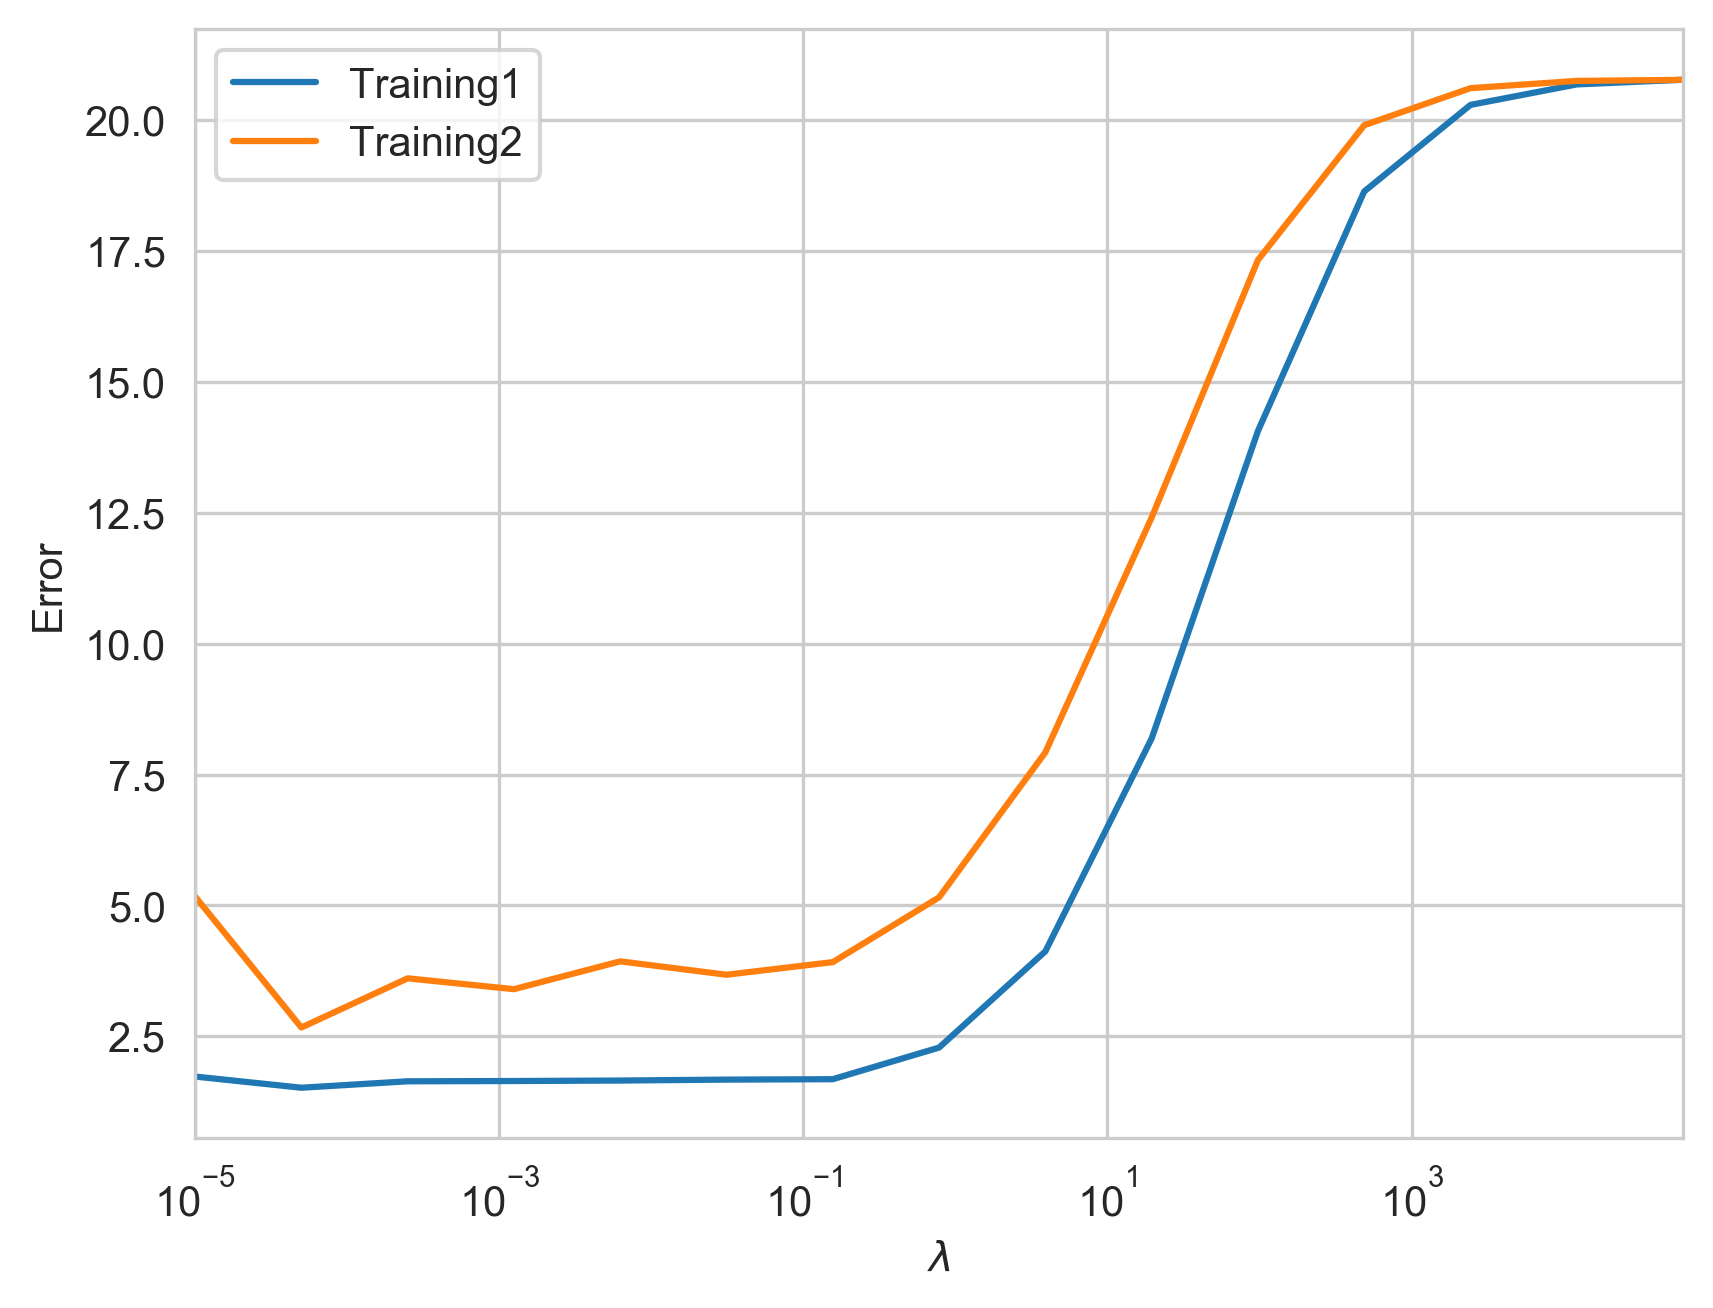
\includegraphics[scale=0.56]{regEout.png}
\caption{Out-of-sample error for different $\lambda$'s.}
\end{figure}

\begin{figure}[h!]
\centering
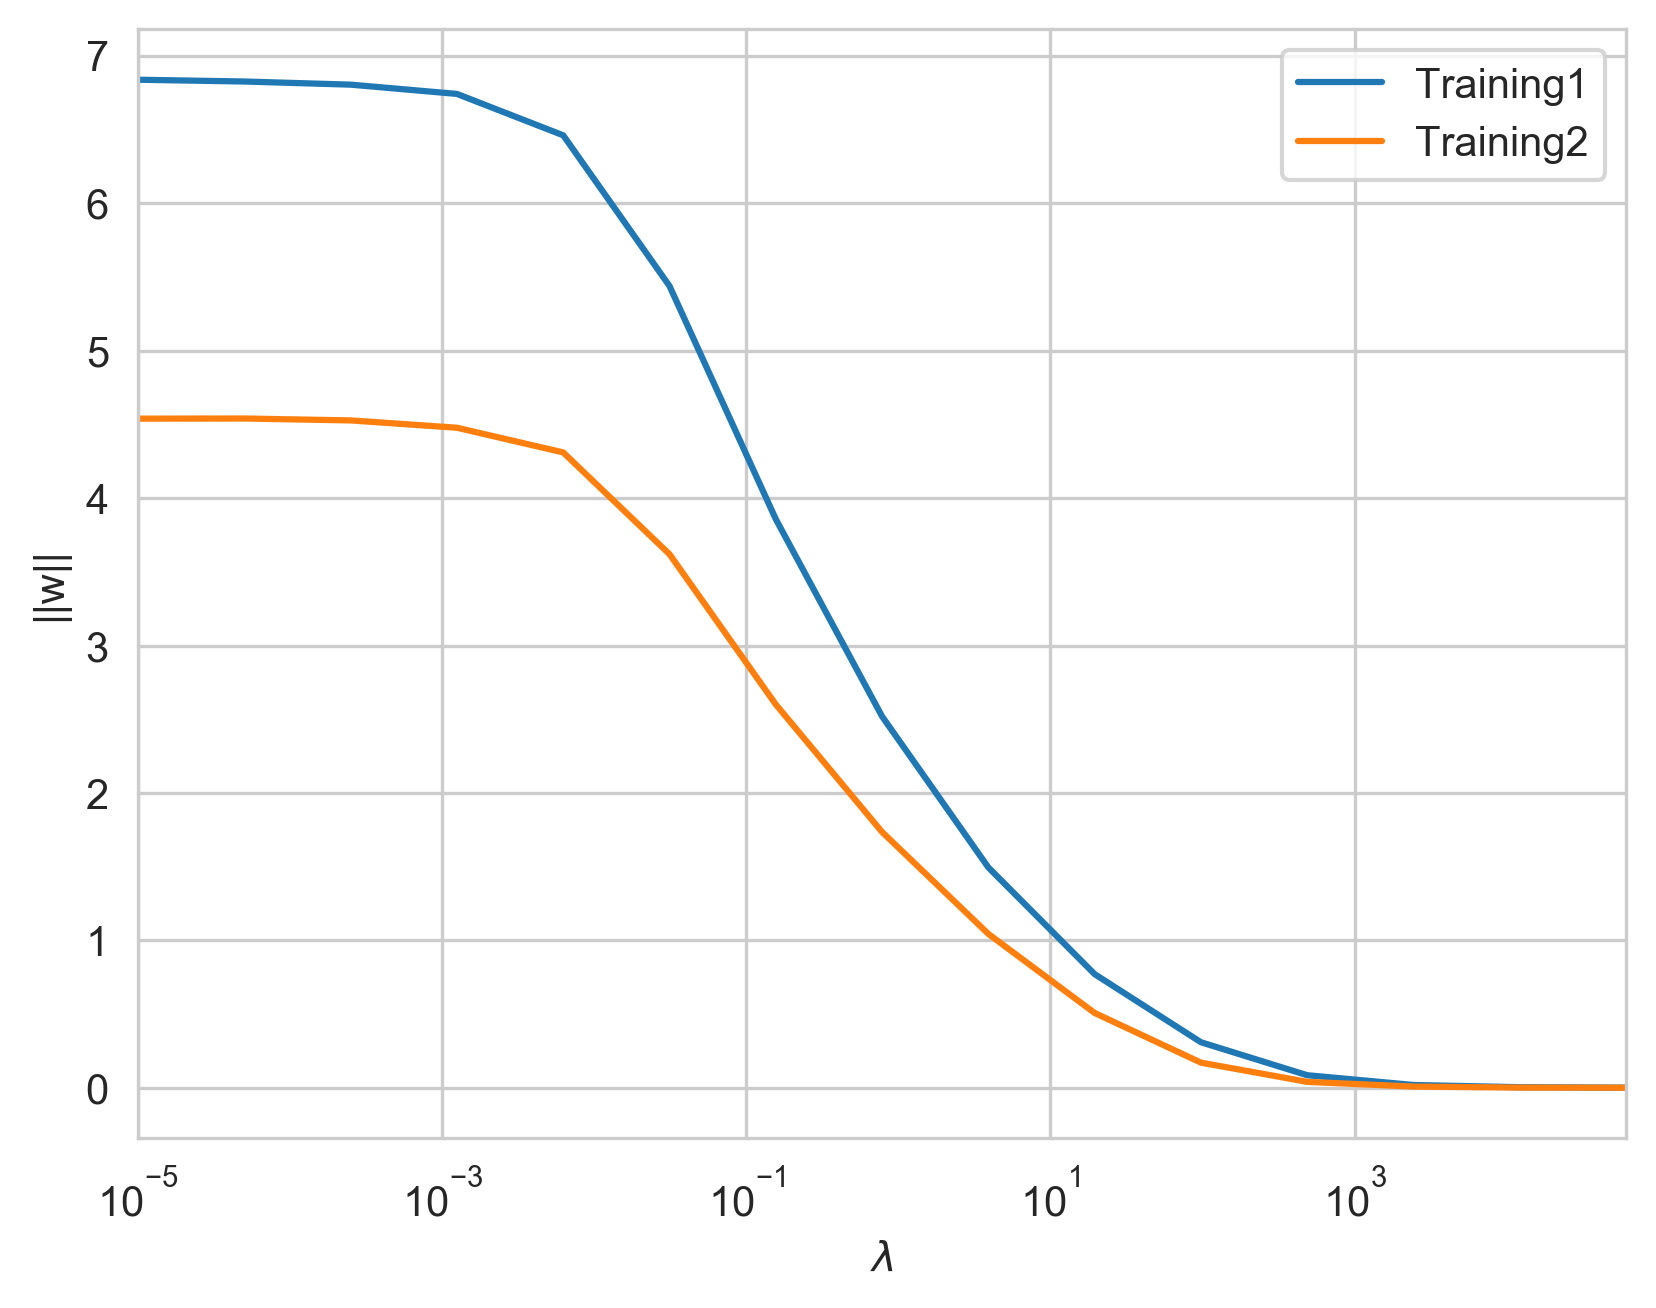
\includegraphics[scale=0.56]{regwnorm.png}
\caption{L2-Norm $||w||$ for different $\lambda$'s.}
\end{figure}

\item The in-sample error is smaller for the subset because there are less points to fit with the logistic model. However, out-of-sample error is larger for the subset because it has less training samples, our estimation of the weights that minimizes out-of-sample has more variance so that our final weight is further from the ideal weight that minimizes the out-of-sample error. Finally, it is clear that the weight norm decrease with a higher $\lambda$ because the regularization term dominates as $\lambda$ increases and then minimizing the loss function essentially becomes minimizing the regularization term. The subset yields a smaller $||w||$ because the loss function is more dominated by the regularization term since the error is summed over less samples, so the training algorithm puts more emphasis on decreasing the regularization term.
\item There is not much of a case of overfitting here. As we reach in the realm of high $\lambda \gg 0.1$, we see that the in-sample error increases dramatically (obviously), but the out-of-sample error also increases dramatically. This is a clear sign of underfitting, implying that high-regularization term restricts the model of the complexity capture in the actual target function.
\item The minimum value of $E_{\text{out}}$ for the Training2 data is $\lambda = 5 \times 10^{-5}$, so I would choose that $\lambda$.
\end{enumerate}
\item
\begin{enumerate}[label = \Alph*.]
\item
\begin{enumerate}
\item We see in Figure \ref{lasso} how the discontinuity and linearity of the L1 norm forces the weights to zero.
\begin{figure}[h!]
\centering
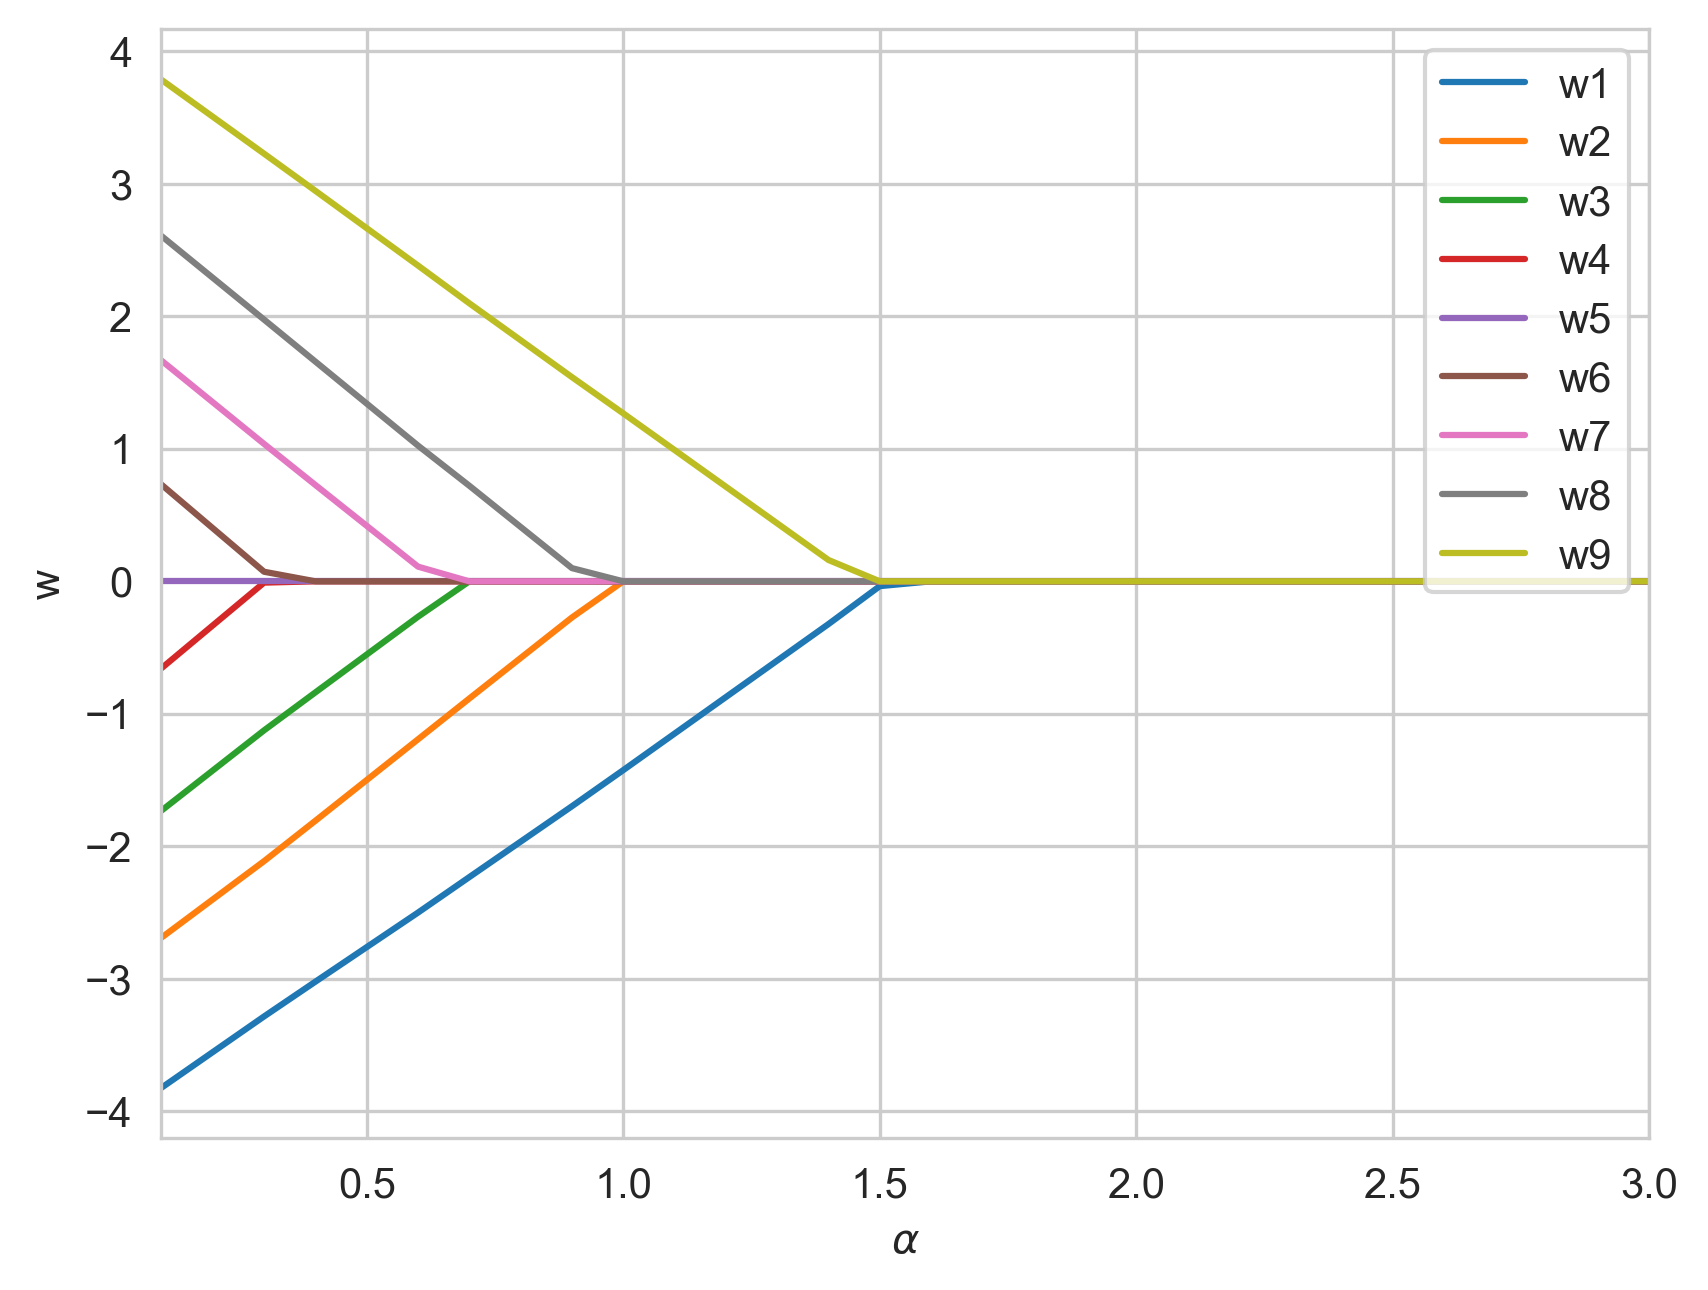
\includegraphics[scale=0.6]{lassoalpha.png}
\caption{Weights versus regularization parameter $\alpha$. For Lasso regularization, the weights quickly die to zero, creating a sparse weight vector.} \label{lasso}
\end{figure}
\item We see in Figure \ref{ridgealpha} that weights don't go to zero, but the norm shrinks to zero as $\alpha \to 0$.
\begin{figure}[h!]
\centering
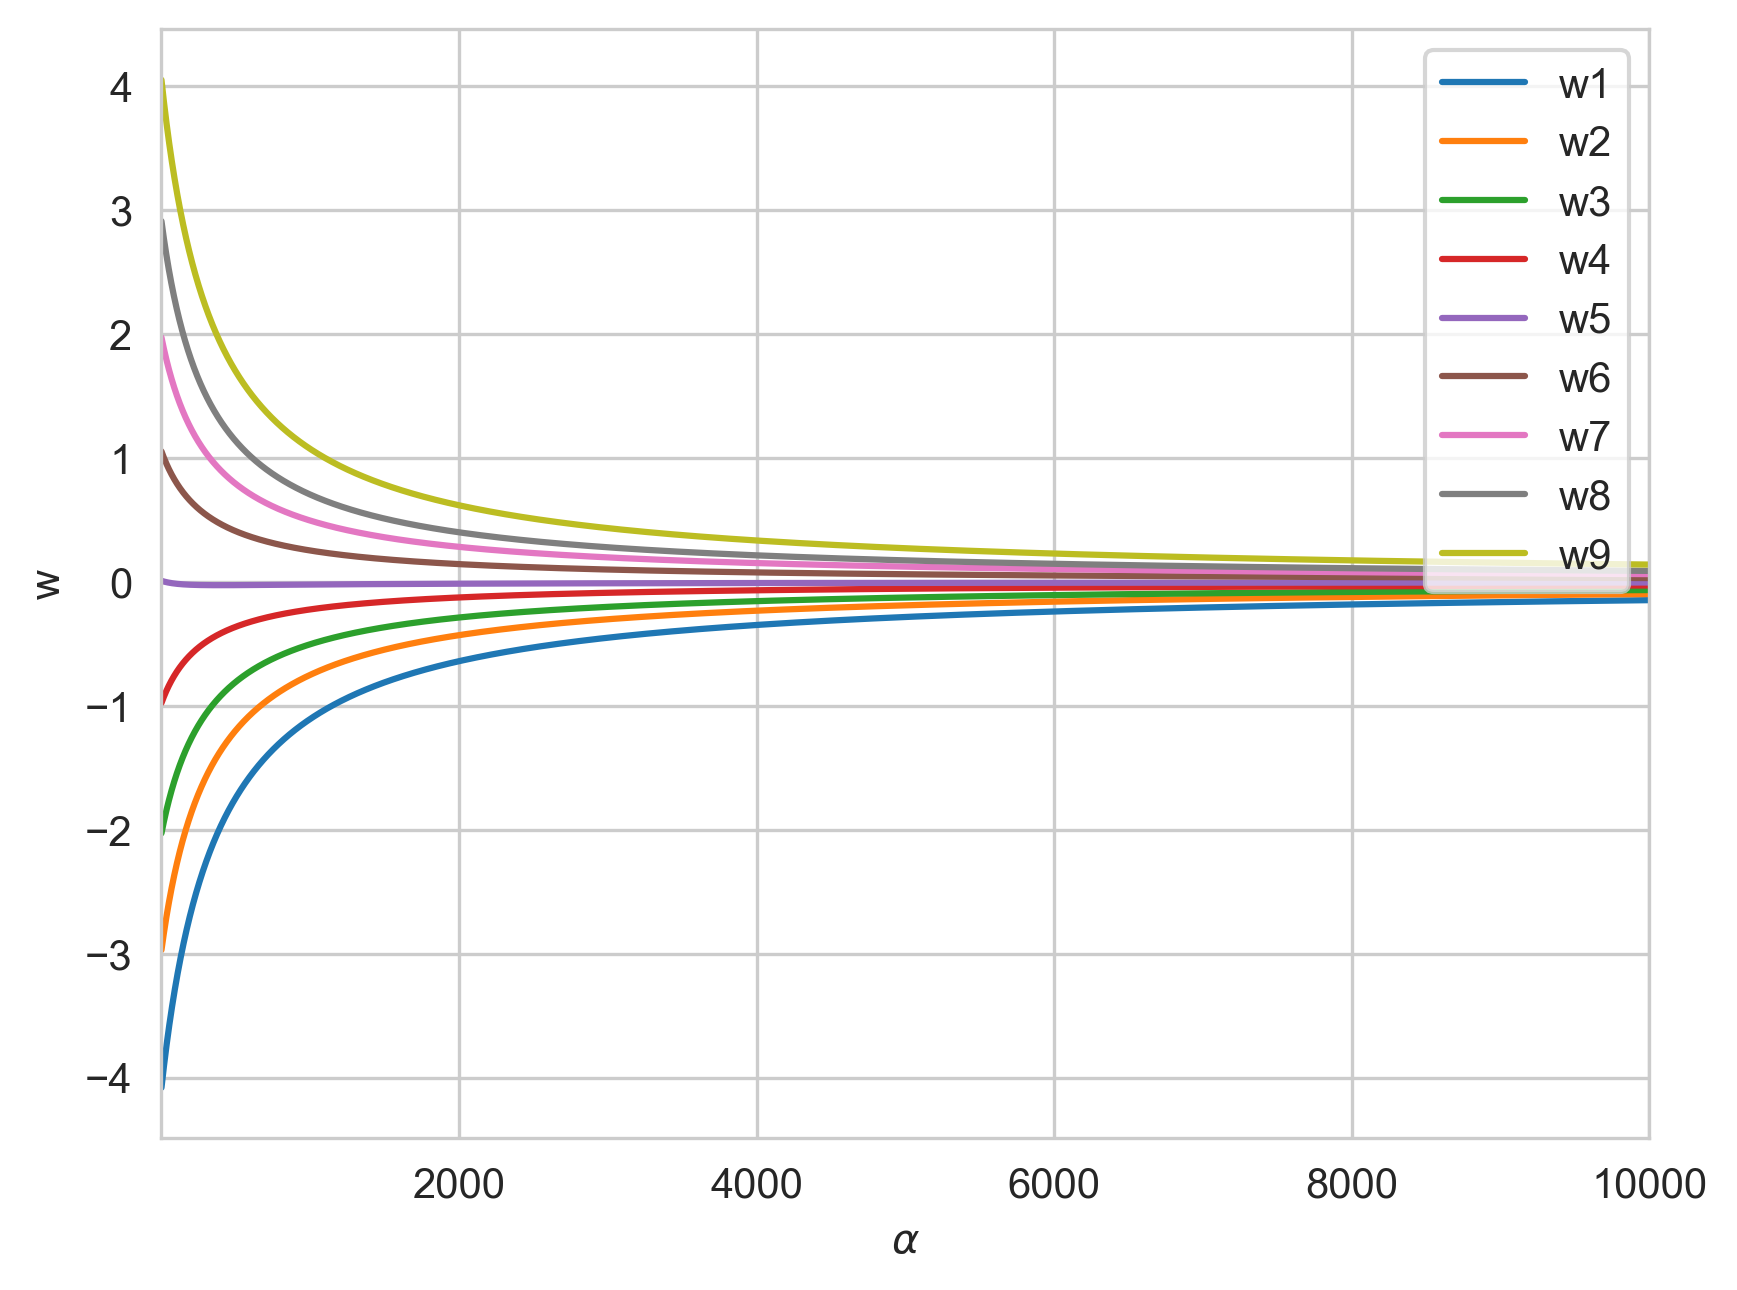
\includegraphics[scale=0.6]{ridgealpha.png}
\caption{Weights verus regularization parameter $\alpha$. For ridge regularization, the weights shrink, but never reach zero, as $\alpha$ increases due to the smoothness of $\w^T \w$.} \label{ridgealpha}
\end{figure}

\item As said in parts i and ii, for Lasso, as $\alpha$ increases, the number of model weights that are exactly zero increases. In ridge regression, the weights don't hit exactly zero, but only get smaller as $\alpha$ increases, as expected.
\end{enumerate}
\item
\begin{enumerate}
\item In this case, $w$ is just a scalar, so we need to calculate
\[ \underset{w}{\text{arg min}} \, L = \underset{w}{\text{arg min}} \left( || \y - w \x ||^2 + \lambda |w| \right) \]
Differentiating with respect to $w$ gives
\begin{align*}
-2 \x^T \y + 2 w \x^T \x + \lambda \frac{|w|}{w} &= 0
\end{align*}
The $w > 0$ solution is
\[ w = \frac{1}{2 \x^T \x} \left( 2 \x^T \y - \lambda \right). \]
The $w < 0$ solution is
\[ w = \frac{1}{2 \x^T \x} \left( 2 \x^T \y + \lambda \right), \]
and the $w = 0$ solution is, of course,
\[ w = 0. \]
We have to decide which one minimizes the Lasso error function. In the $w < 0$ case, we have
\begin{align*}
L_{w > 0} &= \bigg| \bigg| \y - \frac{\x^T \y}{\x^T \x} \x + \frac{\lambda \x}{2 \x^T \x} \bigg| \bigg|^2 + \lambda \bigg| \frac{\x^T \y}{\x^T \x} - \frac{\lambda}{2 \x^T \x} \bigg| \\
&= \y^T \y + \frac{(\x^T \y)^2}{\x^T \x} + \frac{\lambda^2}{4 \x^T \x} - 2 \frac{(\x^T \y)^2}{\x^T \x} + \frac{\lambda \x^T \y}{\x^T \x} - \frac{\lambda \x^T \y}{\x^T \x} \\
& \qquad + \lambda \bigg| \frac{\x^T \y}{\x^T \x} - \frac{\lambda}{2 \x^T \x} \bigg| \\
&= \y^T \y - \frac{(\x^T \y)^2}{\x^T \x} + \frac{\lambda^2}{4 \x^T \x} + \lambda \bigg| \frac{\x^T \y}{\x^T \x} - \frac{\lambda}{2 \x^T \x} \bigg|
\end{align*}
If $2 \x^T \y > \lambda$, then
\[ L_{w > 0, 2 \x^T \y > \lambda} = \y^T \y - \frac{(\x^T \y)^2}{\x^T \x} + \frac{\lambda \x^T \y}{\x^T \x} - \frac{\lambda^2}{4 \x^T \x} = \y^T \y - \frac{(2 \x^T \y - \lambda)^2}{4 \x^T \x} \]
On the other hand,
\[ L_{w > 0, 2 \x^T \y < \lambda} = \y^T \y - \frac{(\x^T \y)^2}{\x^T \x} - \frac{\lambda \x^T \y}{\x^T \x} + \frac{3\lambda^2}{4 \x^T \x}\]
Similarly,
\[ L_{w < 0} = \y^T \y - \frac{(\x^T \y)^2}{\x^T \x} + \frac{\lambda^2}{4 \x^T \x} + \lambda \bigg| \frac{\x^T \y}{\x^T \x} + \frac{\lambda}{2 \x^T \x} \bigg|. \]
So we have for $2 \x^T \y + \lambda < 0$
\[ L_{w < 0, 2 \x^T \y < -\lambda} = \y^T \y - \frac{(2 \x^T \y + \lambda)^2}{4 \x^T \x} \]
\[ L_{w < 0, 2 \x^T \y > -\lambda} = \y^T \y - \frac{(\x^T \y)^2}{\x^T \x} + \frac{\lambda \x^T \y}{\x^T \x} + \frac{3 \lambda^2}{4 \x^T \x} \]
And finally,
\[ L_{w = 0} = \y^T \y. \]
Now if $2 \x^T \y > \lambda$, then $L_{w>0, 2\x^T \y > \lambda}$ definitely has the lowest error. If $2 \x^T \y < - \lambda$, then $L_{w < 0, 2 \x^T \y < - \lambda}$ has the lowest error. What happens in the case of $- \lambda < 2 \x^T \y < \lambda$? The $w > 0$ solution yields
\[ \y^T \y - \frac{(\x^T \y)^2}{\x^T \x} - \frac{\lambda \x^T \y}{\x^T \x} + \frac{3\lambda^2}{4 \x^T \x} > \y^T \y - \frac{\lambda^2 + 2 \lambda^2 + 3 \lambda^2}{4 \x^T \x} = \y^T \y \]
and the $w < 0$ solution yields
\[ \y^T \y - \frac{(\x^T \y)^2}{\x^T \x} + \frac{\lambda \x^T \y}{\x^T \x} + \frac{3 \lambda^2}{4 \x^T \x} > \y^T \y - \frac{\lambda^2 - 2 \lambda^2 + 3 \lambda^2}{4 \x^T \x} = \y^T \y. \]
So in this realm, the $L_{w = 0}$ solution wins. Note the continuity of the solutions in $2 \x^T \y$. In summary, we have
\begin{align*}
w = \frac{1}{2 \x^T \x} (2 \x^T \y - \lambda) \qquad &\text{if} \qquad 2 \x^T \y > \lambda \\
w = \frac{1}{2 \x^T \x} (2 \x^T \y + \lambda) \qquad &\text{if} \qquad 2 \x^T \y < - \lambda \\
w = 0 \qquad &\text{if} \qquad - \lambda \leq 2 \x^T \y  \leq \lambda.
\end{align*}
\item And of course, the smallest value of $\lambda$ such that $w = 0$ is $\lambda = |2 \x^T \y|$.
\item Differentiating with respect to $\w$ and setting to zero yields
\[ - 2 \X^T \y + 2 \X^T \X \w + 2 \lambda \w = 0 \]
so
\[ \w = (\X^T \X + \lambda I)^{-1} \X^T \y. \]
\item In one-dimension, our solution becomes
\[ w = \frac{\x^T \y}{\x^T \x + \lambda}. \]
This is not zero unless $\x^T \y = 0$ (which is impossibly rare). Nevertheless, choosing $\lambda$ won't affect whether it's zero or not.
\end{enumerate}
\end{enumerate}
\end{enumerate}

\end{document}